\documentclass{vilniustech}
\vilniustechsetup{
    university={Vilniaus Gedimino technikos universitetas},
    faculty={Fundamentinių mokslų fakultetas},
    cathedral={Matematinės statistikos katedra},
    workTitle={Mokslinių tyrimų ir inovacijų pagrindų},
    workType={Namų darbas nr.1},
    workAuthorGroup={ITSfm-22},
    workAuthorName={Aurimas Šakalys},
    workRecipient={doc. dr. Rūta Simanavičienė}
}
\addbibresource{example.bib}
\VTDocumentBegin

\section{System security assurance: A systematic literature review}

\subsection{Straipsnio bibliografinis aprašas}
\subsection{Kokia mokslinė problema sprendžiama analizuojamame darbe?}
\subsection{Darbo tikslas, keliamas analizuojamame darbe}
\subsection{Uždaviniai, formuluojami analizuojamame darbe}
\subsection{Koks yra mokslinio darbo naujumas}
\subsection{Koks literatūros apžvalgos tipas taikomas?}
\subsection{Koks empirinio tyrimo metodas taikomas?}
\subsection{Kokie statistiniai metodai taikomi duomenų analizei?}
\subsection{Kurį Bloom'o taksonomijos lygmenį atitinka šis mokslinis darbas ir kodėl?}
\subsection{Koks citavimo stilius naudojamas šiame darbe?}
\subsection{Kokioms mokslinių publikacijų citavimo duomenų bazėms priklauso žurnalas, kuriame publikuojamas šis straipsnis?}

\section{Standardizing information security - a structurational analysis}

\subsection{Straipsnio bibliografinis aprašas}
\subsection{Kokia mokslinė problema sprendžiama analizuojamame darbe?}
\subsection{Darbo tikslas, keliamas analizuojamame darbe}
\subsection{Uždaviniai, formuluojami analizuojamame darbe}
\subsection{Koks yra mokslinio darbo naujumas}
\subsection{Koks literatūros apžvalgos tipas taikomas?}
\subsection{Koks empirinio tyrimo metodas taikomas?}
\subsection{Kokie statistiniai metodai taikomi duomenų analizei?}
\subsection{Kurį Bloom'o taksonomijos lygmenį atitinka šis mokslinis darbas ir kodėl?}
\subsection{Koks citavimo stilius naudojamas šiame darbe?}
\subsection{Kokioms mokslinių publikacijų citavimo duomenų bazėms priklauso žurnalas, kuriame publikuojamas šis straipsnis?}

\section{Literatūra}

\section{Citavimo pavyzdžiai}

\subsection{Įvairių objektų citavimas}

Tinklalapio citavimas \parencite{webcitation}.
\begin{verbatim}
    \parencite{webcitation}
\end{verbatim}

Straipsnio citavimas \parencite{articlecitation}.
\begin{verbatim}
    \parencite{articlecitation}
\end{verbatim}

Knygos citavimas \parencite{bookcitation}.
\begin{verbatim}
    \parencite{bookcitation}
\end{verbatim}


\subsection{Citavimo komandos}

Parastas citavimas \cite{articlecitation}.
\begin{verbatim}
    \cite{articlecitation}
\end{verbatim}

Citavimas skliausteliuose \parencite{articlecitation}.
\begin{verbatim}
    \parencite{articlecitation}
\end{verbatim}

Citavimas poraštėje \footcite{articlecitation}.
\begin{verbatim}
    \footcite{articlecitation}
\end{verbatim}

Citavimas tekstu \textcite{articlecitation}.
\begin{verbatim}
    \textcite{articlecitation}
\end{verbatim}

\newpage
\section{Iliustracijų/lentelių pavyzdžiai}

\begin{figure}[H]
\begin{center}
    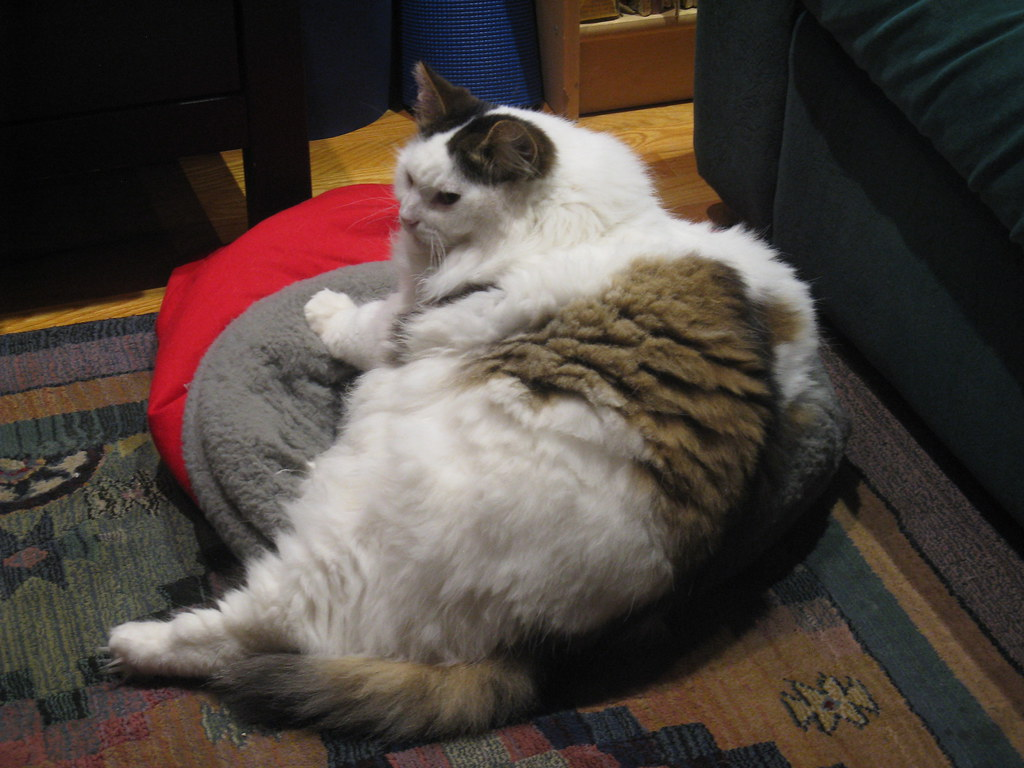
\includegraphics[height=6cm]{img/chonker.jpg}
    \caption{Gabalainis}
    \label{fig:fig1}
\end{center}
\end{figure}

\VTTable{[
    caption = {Trumpa lentelė},
    label = {table:short}
    ]{
    colspec = {XX},
    row{1} = {font=\bfseries}
    }
    Antraštė 1 & Antraštė 2 \\
    Lorem ipsum & Lorem ipsum \\
    Lorem ipsum & Lorem ipsum \\
}

\subsection{Nuorodos}

Nuoroda į iliustraciją \ref{fig:fig1} esančią \pageref{fig:fig1} puslapyje.
\begin{verbatim}
    \ref{fig:fig1} \pageref{fig:fig1}
\end{verbatim}

Nuoroda į trumpą lentelę \ref{table:short} esančią \pageref{table:short} puslapyje.
\begin{verbatim}
    \ref{table:short} \pageref{table:short}
\end{verbatim}

Nuoroda į ilgą lentelę \ref{table:long} esančią \pageref{table:long} puslapyje.
\begin{verbatim}
    \ref{table:long} \pageref{table:long}
\end{verbatim}

\VTTable{[
    caption = {Kelių puslapių lentelė},
    label = {table:long}
    ]{
    colspec = {XXX},
    rowhead = 1,
    row{1} = {font=\bfseries}
    }
    Antraštė 1 & Antraštė 2 & Antraštė 3 \\
    Lorem ipsum & Lorem ipsum & Lorem ipsum \\
    Lorem ipsum & Lorem ipsum & Lorem ipsum \\
    Lorem ipsum & Lorem ipsum & Lorem ipsum \\
    Lorem ipsum & Lorem ipsum & Lorem ipsum \\
    Lorem ipsum & Lorem ipsum & Lorem ipsum \\
    Lorem ipsum & Lorem ipsum & Lorem ipsum \\
    Lorem ipsum & Lorem ipsum & Lorem ipsum \\
    Lorem ipsum & Lorem ipsum & Lorem ipsum \\
    Lorem ipsum & Lorem ipsum & Lorem ipsum \\
}

\VTDocumentEnd